\chapter{Ionización de moléculas biológicas}

\section{Introducción}

El daño causado por el impacto de projectiles pesados cargados en blancos
biológicos se ha convertido un campo de interés debido a su reciente
implementación en la terapia contra el cáncer que implementa haces de 
iones. La efectividad de la radiación depende de la elección de los iones
a implementar. En particular, estudios teóricos y experimentales con
diferentes projectiles han concluido que los iones cargados de carbón 
podrían ser los iones más apropiados para dicha 
implementación~\cite{Mohamad2017}. Sin embargo, el estudio de tales 
sistemas representa un desafío desde el punto de vista teórico.

La ionización de moléculas biológicas por iones de carga múltiple 
constituye el principal mecanismo de daño. El método utilizado con mayor
frecuencia para predecir tales procesos es la primera aproximación de 
Born. A altas energías, este método perturbativo garantiza las leyes de
$Z^2$, donde $Z$ es la carga del projectil. Sin embargo, el daño está 
concentrado en los alrededores del pico de Bragg --a energías de unos 
cientos de keV/amu--, precisamente donde la aproximación de Born empieza
a fallar. Otra dificultad teórica surge de la propia descripción de 
los blancos; estamos tratando con moleculas complejas, y la descripción
de tales blancos representa una tarea difícil para cálculos de primeros
principios.

Se han propuesto diferentes aproximaciones para lidear con la ionización
blancos moleculares dentro del modelo de átomo independiente. Por ejemplo,
en el trabajo propuesto por Galassi~\textit{et al.}~\cite{galassi2000} se
obtienen secciones eficaces moleculares combinando resultados atómicos 
basados en el método de Continuum Distorted Wave-Eikonal Initial State
(\acs{cdw}) y la población de los orbitales moleculares. Más recientemente,
L\"udde~\textit{et al.}~\cite{ludde2016,ludde2018} propone la combinación
de secciones eficaces atómicas con correcciones geométricas de 
apantallamiento.

En este capítulo lidiaremos con dos aspectos de la ionización de moléculas
biológicas; primero, se realizarán cálculos más apropiados para representar
el mecanismo de daño principal, que reemplace los resultados obtenidos
mediante el método de Born. En segundo lugar, estudiaremos la 
implementación de un modelo estequiométrico para describir la ionización
de blancos moleculare.
 
Para superar las limitaciones de las aproximaciones perturbativas de 
primer orden, y dado que los projectiles son iones de carga múltiple, 
implementaremos el método 
CDW~\cite{galassi2000,fainstein1988,miraglia2008,miraglia2009}, el 
cual incluye correciones perturbativas de mayor orden. Detalles sobre 
el método y los cálculos se encuentran en la sección~\ref{sec:atoms}.
Basamos nuestro trabajo en la premisa de que el proceso de ionización 
es el mecanismo que deposita la mayor cantidad de energía primaria en el
sistema. Más aún, se conoce que los electrones residuales de la ionización
son una fuente significativa de daño biológico local~\cite{Denifl2011}. 
Los electrones secundarios son incluidos en simulaciones de Monte Carlo,
y por lo tanto su comportamiento requiere especial atención.
En la sección~\ref{subsec:meanener} y \ref{subsec:meanang}, estudiamos
las distribuciones energéticas y angulares medias de los electrones 
ejectados. Contrariamente a lo esperado según la primera aproximación 
de Born, encontramos que una dependencia sustancial con la carga del 
projectil. 

En la sección~\ref{sec:SSM}, tratamos la complejidad de la estructura 
molecular de los blancos implementando el modelo estequiométrico simple 
(\acs{ssm}), el cual consiste en asumir que las moleculas están 
compuestas por átomos aislados e independientes, y que la sección eficaz 
se expresa como una combinación lineal de cálculos atómicos pesados según 
la estequiometría de la molécula. Así, implementando en conjunto el 
método CDW y SSM, podemos obtener las secciones eficaces de ionización de 
diversas moléculas de interés biológico, incluyendo las moléculas que 
componen el ADN y ARN --adenina, citosina, guanina, timina, uracilo--, 
tetrahidrofurano (\acs{thf}), pirimidina y grupos de fosfato del 
esqueleto del ADN, debido al impacto de antiprotones, H$^{+}$, He$^{2+}$, 
Be$^{4+}$, C$^{6+}$, y O$^{8+}$. 
En la sección~\ref{sec:scaling}, estudiamos la regla de escala de 
Toburen~\cite{toburen1975,toburen1976}, que establece que la razón entre
la sección eficaz de ionización y el número de electrones débilmente
ligados se puede ubicar sobre una delgada banda universal en términos 
de la velocidad del projectil. Aplicamos esta regla para un número 
significativo de hidrocarburos y nucleobases, notando que el ancho de las
bandas resultantes puede ser reducida significativamente si consideramos
el número de electrones activos en la colisión basándonos en los 
cálculos según el método CDW de los diferentes átomos constituyentes. 
La regla de escala resultante es implementada teóricamente y comparada 
con datos experimentales disponibles.

La aproximación SSM considera los átomos en una molécula como si fueran
neutrales, lo cual no es correcto. En la sección~\ref{sec:molcalculations}, 
usaremos cálculos de estructura molecular realizados con el código
{\sc gamess}~\cite{gamess} para calcular el exceso o defecto de densidad 
electrónica en los átomos que componen las moléculas. Así, modificamos
la formula estequimétrica para tener en cuenta el alejamiento de la 
neutralidad de los átomos. Encontramos que modificación a la aproximación 
SSM para las moléculas de ADN no introduce cambios sustanciales en las 
secciones eficaces totales de ionización.

%%%%%%%%%%%%%%%%%%%%%%%%%%%%%%%%%%%%%%%%%%%%%%%%%%%%%%%%%%%%%%%%%%%%%%%%
\section{Ionización de átomos constituyentes}
\label{sec:atoms}
%%%%%%%%%%%%%%%%%%%%%%%%%%%%%%%%%%%%%%%%%%%%%%%%%%%%%%%%%%%%%%%%%%%%%%%%

En esta sección, consideraremos cuatro blancos atómicos: $\alpha=$ H, C, 
N y O, y seis proyectiles: antiprotones $\bar{p}$, H$^{+}$, He$^{2+}$, 
Be$^{4+}$, C$^{6+}$, y O$^{8+}$. La mayor parte de las moléculas organicas 
están compuestos por estos átomos. Algunas moléculas en particular están 
compuestas por halógenos tales como flúor o bromo. Las secciones eficaces 
de estos átomo han sido calculadas y publicadas por 
Miraglia~\cite{miraglia2008}.

La sección de ionización total de estos átomos $\sigma_{\alpha}$ se
calculan usando la aproximación CDW. Los funciones de onda radiales
de los estados inicial ligado y final continuo se calculan usando el
código {\sc radialf}, desarrollado por Salvat y 
colaboradores~\cite{salvat1995}, implementando potenciales efectivos que
se obtienen a partir del método de Inversión Depurada desarrollado en el
capítulo anterior~\cite{Mendez:16,Mendez:18}. Usamos un par de miles
de puntos como pivotes para resolver la ecuación de Schr\"{o}dinger,
dependiendo del número de oscilaciones del estado del contínuo. 
La integración radial fue realizada usando la técnica de interpolación
cúbica. Expandimos las función de onda del estado final en el continuo
como
\begin{equation}
\psi_{\overrightarrow{k}}^{-}(\overrightarrow{r})=\sum_{l=0}^{l_{\max
}}\sum_{m=-l}^{l}R_{kl}^{-}(r)Y_{l}^{m}(\widehat{r})Y_{l}^{m^{\ast }}
(\widehat{k})\,.
\label{eq:contwave}
\end{equation}
El número de momentos angulares considerados variaron desde 8, para 
electrones expulsados a muy bajas energías, hasta $l_{\max}\sim 30$, 
para las energías más altas consideradas. Se requirieron el mismo 
número de ángulos azimutales para obtener las secciones eficaces 
diferenciales cuádruples. El cálculo realizado no muestra discrepancias 
en las versiones posteriores y previas del método. Cada sección eficaz
atómica total fue calculada usando entre 35 y 100 valores de 
transferencia de momento, 28 ángulos electrónicos fijos, y alrededor
de 45 valores de energía electrónica, dependiendo de la energía de 
impacto del proyectil. Para más detalle, se puede consultar el trabajo
publicado por Montanari en la Ref.~\cite{montanari2017}. 

\begin{figure}
\centering
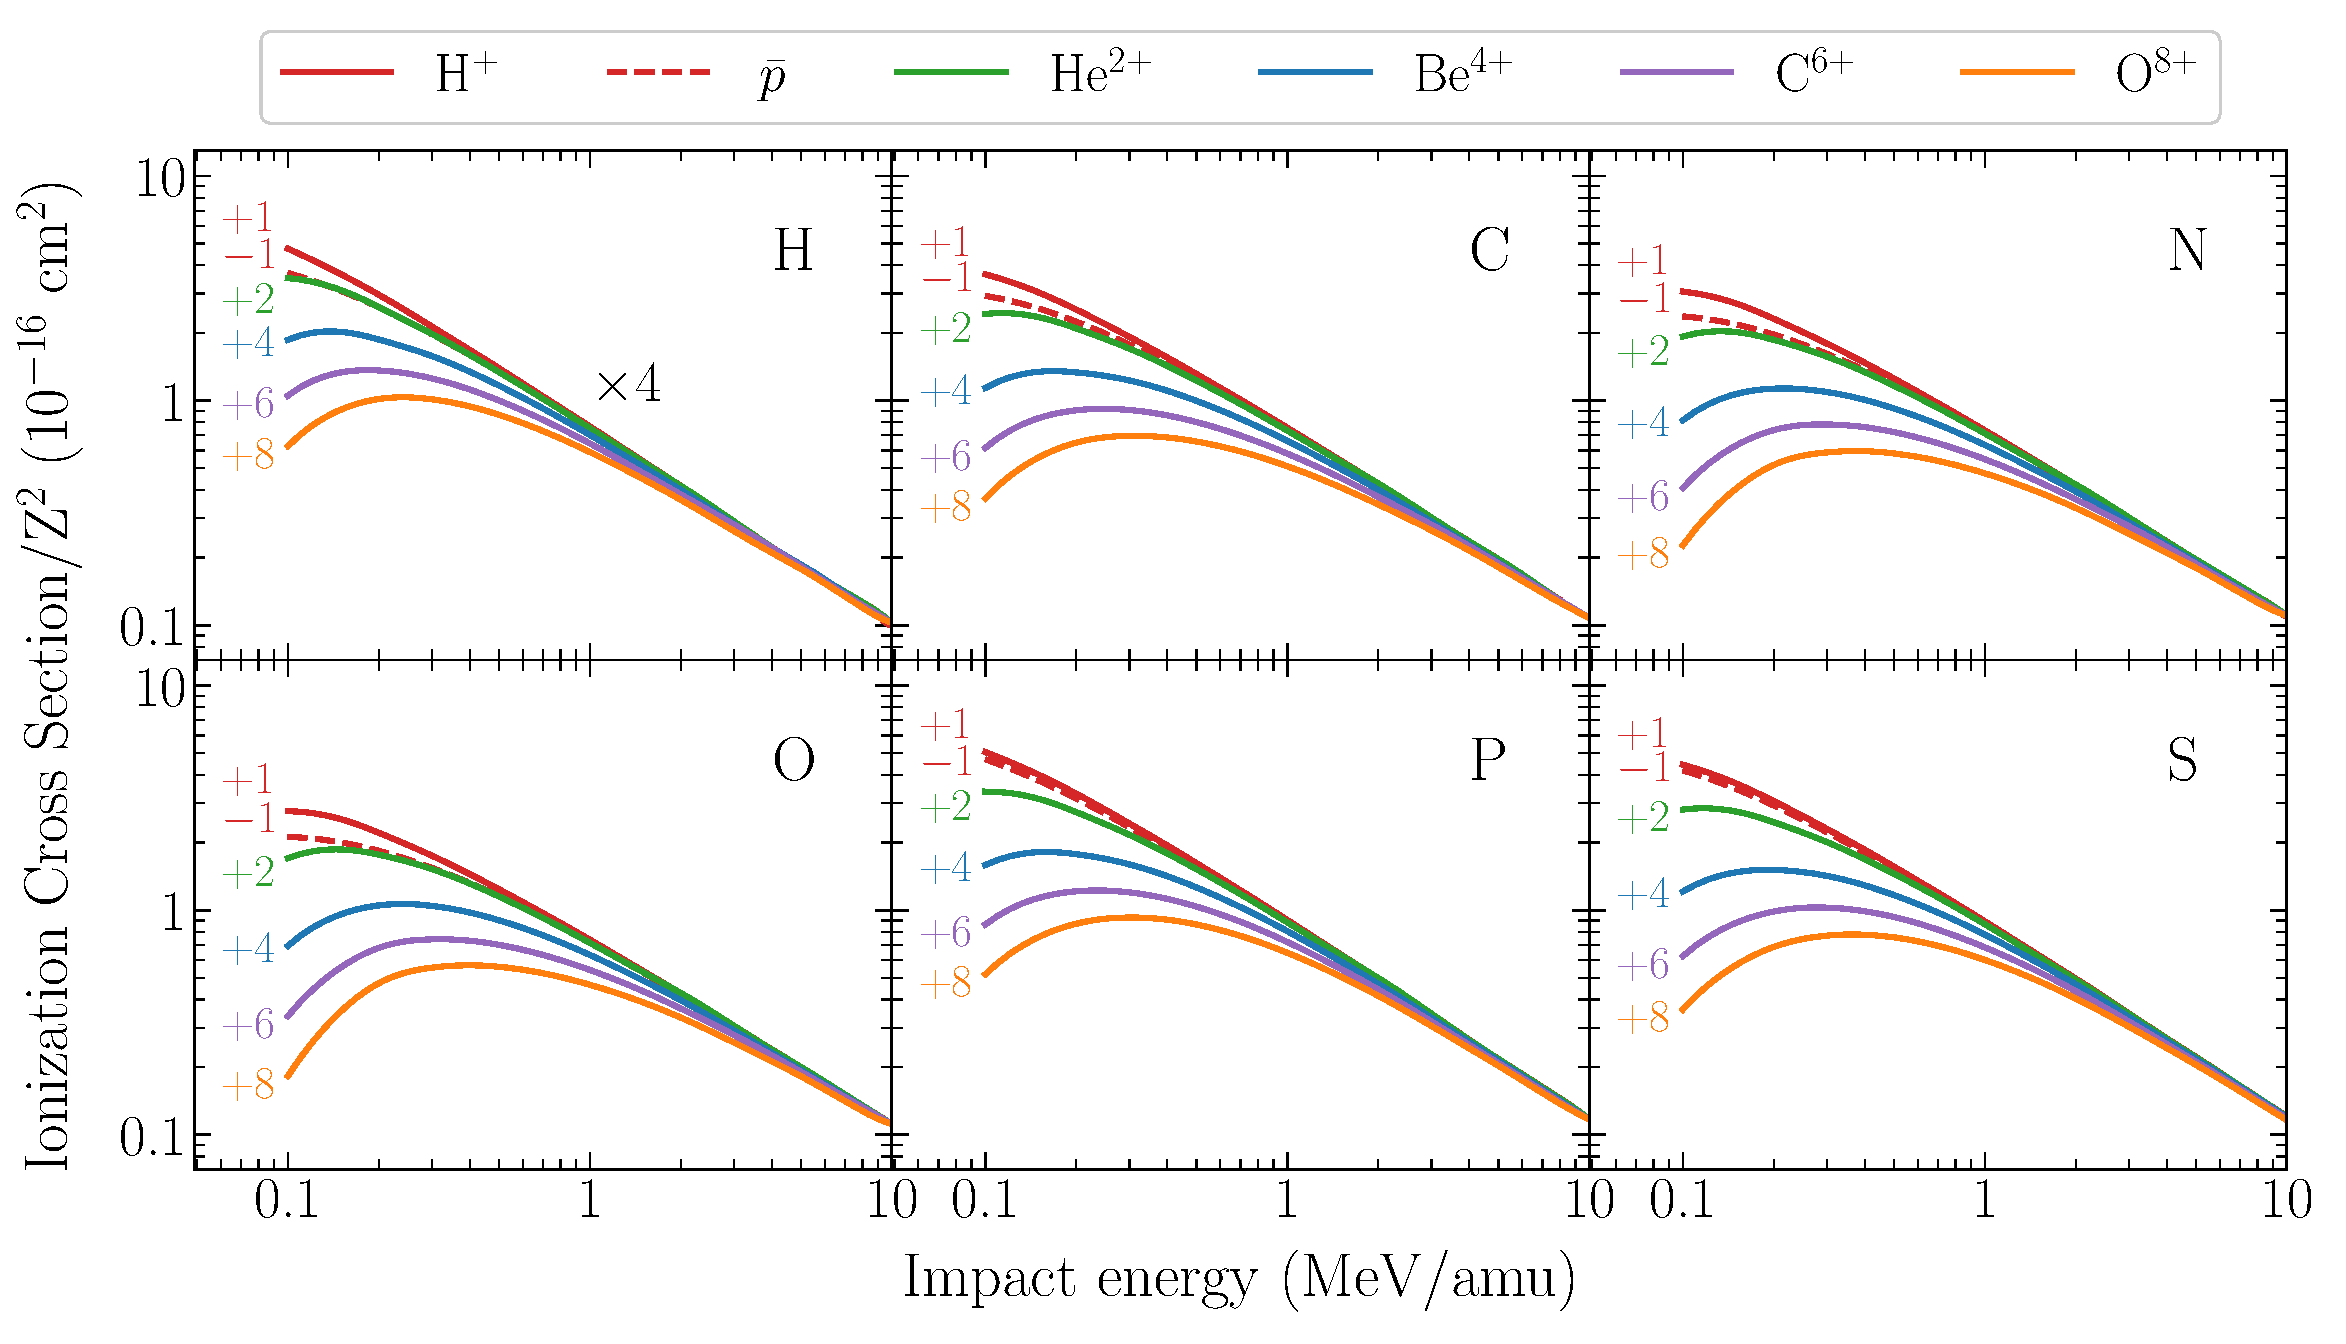
\includegraphics[width=0.9\textwidth]{ionmol/atomicscaling.eps}
\caption[Sección eficaz total de ionización reducida de átomos relevantes.]
{Sección eficaz total de ionización CDW reducida $\sigma_{\alpha}/Z^2$ 
de cuatro blancos atómicos relevantes. Las curvas se corresponden a los 
estados de carga de los seis proyectiles. Experimentos: 
\mbox{\Large$\circ$} ionización de H por impacto de H$^+$~\cite{Shah:81};
ionización por impacto de electrones en $\rhd$ H~\cite{Shah:87}, 
$\square$ C~\cite{Brook:78}, $\square$ N~\cite{Brook:78} y 
$\triangle$ O~\cite{Thompson:95}.}
\label{fig:atomscaling}
\end{figure} 

En la figura~\ref{fig:atomscaling} mostramos nuestras secciones eficaces
de ionización implementando el método de CDW para cuatro elementos 
esenciales debido al impacto de seis proyectiles cargados. Para comparar 
los 24 sistemas blanco--proyectil resultantes en una única figura, 
consideramos el hecho que en la primera aproximación de Born, la sección 
eficaz de ionización escala con el cuadrado de la carga del proyectil, es 
decir $Z^{2}$. Las energías de impacto consideradas van de 0.1 a 10 MeV/amu, 
donde se supone que el método CDW tiene validez. Nuestros resultados se
comparan con secciones eficaces experimentales para el caso de ionización 
de H por impacto de H$^+$~\cite{Shah:81}. En el rango de medias a altas
energías, se compara la ionización por impacto de electrones, con la 
correspondiente conversión de equivelocidad para energías incidentes de 
electrones superiores a 300 eV, en H~\cite{Shah:87}, C~\cite{Brook:78}, 
N~\cite{Brook:78} y O~\cite{Thompson:95}. De hecho, para los proyectiles 
de carga más altas, el valor de energía mínimo donde se espera que la CDW 
tenga validez es mayor a 100 keV. También realizamos cálculos similares 
con la primera aproximación de Born (no se muestran aquí), y corroboramos 
que ésta provee resultados confiables para valores de energía mayores a 
unos cuantos MeV/amu. Usamos el mismo color de línea para indicar la 
carga del proyectil en todas las figuras que se muestran en este 
capítulo: discontinua--roja, sólida--roja, azul, magenta, oliva y naranja 
para antiprotones, H$^{+}$, He$^{2+}$, Be$^{4+}$, C$^{6+}$, y O$^{8+}$, 
respectivamente. Notablemente, no existen publicaciones en donde se
tabulen la ionización de átomos por impacto de iones cargados.

%%%%%%%%%%%%%%%%%%%%%%%%%%%%%%%%%%%%%%%%%%%%%%%%%%%%%%%%%%%%%%%%%%%%%%%%
\subsection{Distribución energética de electrones}
\label{subsec:meanener}
%%%%%%%%%%%%%%%%%%%%%%%%%%%%%%%%%%%%%%%%%%%%%%%%%%%%%%%%%%%%%%%%%%%%%%%%

En un medio biológico dado, la ionización directa debido al impacto de
un ion representa solo una fracción del daño total. Los electrones
secundarios, así como el retroceso de los iones del blanco, también
contribuyen sustancialmente al daño total~\cite{Denifl2011}. 
Podemos considerar que la sección eficaz de ionización diferencial de la
capa $nl$ del átomo $\alpha$, $d\sigma_{\alpha nl}/dE$, es una función 
de la energía del electrón eyectado $E$ como una función de distribución
simple~\cite{surdutovic2018}. Así, podemos definir una valor medio 
$\overline{E}_{\alpha}$ como el dado por Abril y 
coloboradores~\cite{abril2015},
\begin{eqnarray}
\overline{E}_{\alpha} &=&\frac{\langle E_{\alpha}\rangle}{\langle
1\rangle}=\frac{1}{\sigma_{\alpha}}\sum\limits_{nl}\int dE\,E
\frac{d\sigma_{\alpha,nl}}{dE}\,,  
\label{40} \\
\langle 1\rangle &=&\sigma_{\alpha}=\sum\limits_{nl}\int dE\,
\frac{d\sigma_{\alpha,nl}}{dE}\,. 
\label{50}
\end{eqnarray}
donde $\Sigma_{nl}$ tiene en cuenta la suma de las diferentes 
contribuciones de cada capa del elemento $\alpha$.

\begin{figure}
\centering
\includegraphics[width=0.9\textwidth]{ionmol/ener_mean.eps}
\caption[Distribución energética media de electrones emitidos.]
{Distribución energética media de electrones emitidos por ionización 
debido al impacto de iones cargados dado por la ecuación~(\ref{40}). 
La línea punteada corresponde a la aproximación de Born con $Z=1$.
La línea discontinua y las líneas sólidas hacen referencia a $\bar{p}$ e 
iones de carga $+1$, $+2$, $+4$, $+6$ y $+8$, respectivamente.}
\label{fig:emittedener}
\end{figure*} 

Las energías medias de los electrones emitidos $\overline{E}_{\alpha}$ 
para H, C, N y O se muestran en la figura~\ref{fig:emittedener}. 
El rango de velocidad de impacto fue reducido a $v=10$~a.u. debido 
a las limitaciones numéricas en la expansión de esféricos armónicos dados
por la ecuación~(\ref{eq:contwave}). A medida que la velocidad de 
impacto $v$ aumenta, también aumenta $\langle E_{\alpha}\rangle$ y
$l_{\max}$, lo que resulta en la inclusión de funciones con muchas 
oscilaciones en el integrando. Más aún, el integrando de 
$\langle E_{\alpha}\rangle$ incluye energías cinéticas $E$
(ver ecuación~(\ref{40})), que cancela la región de energía pequeña y 
refuerza los valores grandes, haciendo que el resultado sea más 
sensible a los momentos angulares mayores. Independientemente, para 
$v>10$ a.u., la primera aproximación de Born es válida. 

En la figura~\ref{fig:emittedener}, estimamos $\overline{E}_{\alpha}$ de
los electrones emitidos en el rango de energía de 10 a 70 eV, para 
todos los blancos. Nuestros resultados concuerdan con los hallazgos 
experimentales~\cite{surdutovic2018}. Como se puede observar en la 
figura, el valor de energía media es sorprendentemente sensible a la 
carga del proyectil $Z$, que puede duplicar los resultados de protón en 
la región intermedia, i.e., 100--400 keV/amu. El efecto observado puede 
atribuirse al repulsión electrónica causada por los iones de carga 
múltiple en los electrones de baja energía. Este comportamiento no se 
puede encontrar en la primera aproximación de Born, donde la ley de
escala $Z^2$ cancela la dependencia con $Z$ de la ecuación~(\ref{40}).
A altas energías, $\overline{E}_{\alpha}$ tiende a un valor universal
para todos los iones, como puede verse en la figura~\ref{fig:emittedener}.

%%%%%%%%%%%%%%%%%%%%%%%%%%%%%%%%%%%%%%%%%%%%%%%%%%%%%%%%%%%%%%%%%%%%%%%%
\subsection{Distribución angular de electrones}
\label{subsec:meanang}
%%%%%%%%%%%%%%%%%%%%%%%%%%%%%%%%%%%%%%%%%%%%%%%%%%%%%%%%%%%%%%%%%%%%%%%%

\begin{figure}
\centering
\includegraphics[width=0.9\textwidth]{ionmol/ang_mean.eps}
\caption[Distribución angular media de electrones emitidos.]
{Distribución angular media de electrones emitidos por ionización debido
al impacto de iones cargados. Las curvas son iguales a las de la 
figura~\ref{fig:emittedener}.}
\label{fig:emittedang}
\end{figure} 

Como mencionamos anteriormente la emisión de electrones secundarios
contribuye al daño total. Entonces, no sólo es esencial conocer la 
distribución de energía de los electrones eyectados, sino también la 
dirección a la que los electrones son emitidos. Una vez más, podemos
considerar que la sección eficaz diferencial de ionización, que se 
escribe en términos del ángulo sólido de eyección del electrón $\Omega$, 
$d\sigma_{\alpha,nl}/d\Omega$, puede expresarse como una función de 
distribución. Así, el ángulo medio de emisión $\overline{\theta}_{\alpha}$ 
se puede definir como
\begin{eqnarray}
\overline{\theta}_{\alpha}&=&\frac{\langle\theta_{\alpha}\rangle}
{\langle 1\rangle}=\frac{1}{\sigma_{\alpha}}\sum\limits_{nl}
\int d\Omega\,\theta\,\frac{d\sigma_{\alpha,nl}}{d\Omega} \\
\langle 1\rangle &=&\sigma_{\alpha}=\sum\limits_{nl}\int d\Omega\,
\frac{d\sigma_{\alpha,nl}}{d\Omega}\,.
\end{eqnarray}

Los ángulos medios de emisión electrónica $\overline{\theta}_{\alpha}$ 
ára los seis átomos y los seis iones estudiados aquí se muestran en la 
figura~\ref{fig:emittedang}. Se puede observar una dependencia 
significativa de $\overline{\theta}_{\alpha}$ con $Z$ para todos los 
sistemas colisionales. Una vez más, este efecto no puede ser notado en 
la implementación de FBA (línea punteada).

Para la emisión de electrones de baja energía, la dispersión angular 
es casi isotrópica~\cite{Rudd1992}. Un valor típico para el ángulo de 
eyección considerado en la literatura es 
$\overline{\theta}_{\alpha}\sim$~70\textdegree~\cite{surdutovic2018}, el cual
resulta bastante certero en el rango de validez de la primera 
aproximación de Born para cualquier objetivo. Sin embargo, cuando se 
usa una aproximación de onda distorsionada, $\overline{\theta}_{\alpha}$
disminuye sustancialmente con $Z$ en la región de energía intermedia, 
como se muestra en la figura~\ref{fig:emittedang}. Cuanto mayor sea la 
carga $Z$, menor será $\overline{\theta}$. Por supuesto, este efecto 
solo es válido en energías intermedias y no en energías de alto impacto.

Para ilustrar este rasgo, considere el impacto de C$^{6+}$ con una 
energía de 500~keV sobre oxígeno. La primera aproximación de Born 
predice electrones emitidos con energías medias de 46,7 eV y ángulos 
medios de 78\textdegree, mientras que la aproximación CDW establece 
energías medias de 62,5 eV y un ángulo de emisión igual a 60\textdegree. 
Estos resultados implican una penetración más profunda de los electrones 
secundarios con una orientación más cercana a la dirección del ion. 
Podemos atribuir esta corrección de la dirección de avance a la captura 
del efecto continuo.

Además, la figura~\ref{fig:emittedang} proporciona una descripción 
ilustrativa del comportamiento de los antiprotones: el proyectil repele 
los electrones, siendo $\overline{\theta}_{\alpha}\sim$~90\textdegree. 
Nótese el efecto opuesto de protones y antiprotones con respecto a la 
primera aproximación de Born; este fenómeno constituye un efecto Barkas 
angular.

%%%%%%%%%%%%%%%%%%%%%%%%%%%%%%%%%%%%%%%%%%%%%%%%%%%%%%%%%%%%%%%%%%%%%%%%
\section{El modelo estequiométrico}
\label{sec:SSM}
%%%%%%%%%%%%%%%%%%%%%%%%%%%%%%%%%%%%%%%%%%%%%%%%%%%%%%%%%%%%%%%%%%%%%%%%

Consideremos una molécula $M$ compuesta por $n_{\alpha}$ átomos del 
elemento $\alpha$, el modelo estequiométrico aproxima la sección eficaz 
de ionización total de la molécula $\sigma_{M}$ como una suma de 
secciones eficaces de ionización de los átomos aislados $\sigma_{\alpha}$ 
ponderada por $n_{\alpha}$, 
\begin{equation}
 \sigma_{M}=\sum\limits_{\alpha}n_{\alpha}\sigma_{\alpha}\,.  
 \label{eq:sumion}
\end{equation}
Clasificamos los blancos moleculares de nuestro interés en tres 
familias: CH, CHN y ADN, como se muestra en la tabla~\ref{tab:families}.

\begin{table}[t]
\begin{center}
\begin{tabular}{|p{0.05\textwidth}|p{0.8\textwidth}|}
\hline
\multirow{2}{*}{CH} & CH$_4$ (metano), C$_2$H$_2$ (acetileno), 
C$_2$H$_4$ (eteno), C$_2$H$_6$ (etano), \\ & C$_6$H$_6$ (benzene) \\
\hline
\multirow{2}{*}{CHN} & C$_5$H$_5$N (piridina), C$_4$H$_4$N$_2$ (pirimidina), 
C$_2$H$_7$N (dimetilamina), \\ & CH$_5$N (monometilamina) \\
\hline
\multirow{4}{*}{DNA} & C$_5$H$_5$N$_5$ (adenina), C$_4$H$_5$N$_3$O (citosina), 
C$_5$H$_5$N$_5$O (guanina), \\ & C$_5$H$_6$N$_2$O$_2$ (timina),
C$_4$H$_4$N$_2$O$_2$ (uracilo), C$_4$H$_8$O (THF) \\
% & C$_5$H$_{10}$O$_5$P (esqueleto de ADN), C$_{20}$H$_{27}$N$_7$O$_{13}$P$_2$ (ADN seco) \\
\hline
\end{tabular}
\caption[Blancos moleculares estudiados y clasificados en tres familias.]
{Blancos moleculares de interés estudiados en el presente trabajo y 
clasificados en tres familias.}
\label{tab:families}
\end{center}
\end{table}

En la figura~\ref{fig:crossDNA_1} reportamos las secciones eficaces de 
ionización totales reducida $\sigma_M/Z^2$ para adenina, citosina, 
guanina y timina por el impacto de iones de carga múltiple obtenidos 
combinando el SSM dado por la ecuación~(\ref{eq:sumion}) y los 
resultados de la implementación del método CDW. Para adenina, la 
concordancia con los datos experimentales disponibles para el impacto 
de protones~\cite{iriki2011} es excelente. Hasta donde sabemos, no hay 
datos experimentales sobre la ionización por impacto de iones cargados 
para el resto de moléculas. También hemos incluido en esta figura 
mediciones de ionización por impacto de electrones~\cite{rahman2016} 
con la correspondiente conversión de equivelocidad para energías 
incidentes de electrones superiores a 300 eV. En esta región, la 
sección eficaz de ionización por impacto de protones y electrones 
debería coincidir. Aunque las mediciones de impacto de electrones están 
por encima de nuestros hallazgos para todos los objetivos moleculares, 
vale la pena señalar que nuestros resultados concuerdan muy bien con 
otras predicciones teóricas de impacto de 
electrones~\cite{mozejko2003,tan2018}. 

Las secciones eficaces de ionización total reducidas $\sigma_M/Z^2$ 
para uracilo, esqueleto de ADN, pirimidina y THF se muestran en la 
figura~\ref{fig:crossDNA_2}. Para el uracilo, la concordancia con las 
mediciones experimentales de ionización por impacto de protones de 
Itoh~\textit{et al.}~\cite{itoh2013} es buena. Sin embargo, para el 
mismo blanco, nuestra teoría predice secciones eficaces con un factor 
de dos por encima de las mediciones experimentales de ionización de 
Tribedi y colaboradores~\cite{agnihotri2012,agnihotri2013} para el 
impacto de iones de carga múltiple. No obstante, cabe señalar que 
nuestros resultados teóricos coinciden con los cálculos de Champion, 
Rivarola y colaboradores~\cite{agnihotri2012,champion2012}, lo que 
puede indicar algún problema con los valores experimentales.


Para pirimidina, mostramos una comparación de nuestros resultados con 
los datos experimentales de ionización por impacto de protones de 
Wolff~\cite{wolff2014} y también para la ionización por impacto de 
electrones~\cite{bug2017} a altas energías. Las mediciones de impacto 
de electrones concuerdan con nuestros cálculos para energías superiores 
a 500keV. Inesperadamente, las secciones eficaces de ionización por 
impacto de protones son significativamente más bajas que nuestros 
resultados. Una mayor cantidad de experimentos se encuentran disponibles 
para la ionización de la molécula de THF por impacto de 
protones~\cite{wang2016} y de electrones~\cite{bug2017,wolf2019,fuss2009}. 
Los resultados que obtenemos de la combinación del SSM y las secciones
eficaces atómicas CDW muestran un buen acuerdo general con esta data.

A energías de impacto intermedias, la regla $Z^2$ ya no se cumple y se 
pueden considerar otras escalas en esta región. En la 
sección~\ref{sec:scaling} inspeccionaremos algunas de ellas.


%At intermediate impact energies, the $Z^2$ rule no longer holds, and 
%other scalings can be considered in this region. For example, the 
%molecular cross section and ion impact energy can be reduced with the 
%projectile charge $Z$, as suggested in in~\cite{janev1980,dubois2013}. 

\begin{figure}
\centering
\includegraphics[width=0.9\textwidth]{ionmol/adn1.eps}
\caption[Sección eficaz total de ionización reducida de moléculas (parte 1).]
{Sección eficaz total de ionización reducida CDW $\sigma_{M}/Z^2$ como una 
función de la energía de impacto del ion. Experimentos: 
\mbox{\Large$\circ$}~\cite{iriki2011} para impacto de protón y
$\square$~\cite{rahman2016} para impacto de electron con conversión de
equivelocidad.}
\label{fig:crossDNA_1}
\end{figure} 

\begin{figure}
\centering
\includegraphics[width=0.9\textwidth]{ionmol/adn2.eps}
\caption[Sección eficaz total de ionización reducida de moléculas (parte 2).]
{Sección eficaz total de ionización reducida CDW $\sigma_{M}/Z^2$ como una 
función de la energía de impacto del ion. Experimentos: impacto de protón
en $\triangle$ uracilo~\cite{itoh2013}, 
$\bigtriangledown$ pirimidina~\cite{wolff2014} y $\meddiamond$
THF~\cite{wang2016}. Impacto de $\ominus$ C$^{4+}$, $\oplus$ C$^{6+}$, 
O$^{6+}$, F$^{6+}$, y $\otimes$ O$^{8+}$, F$^{8+}$ en
uracilo~\cite{agnihotri2012,agnihotri2013}. 
Símbolos~$\rhd$~\cite{bug2017}, $\lhd$~\cite{wolf2019}, y 
$\medstar$~\cite{fuss2009} para impacto de electrón con conversión de 
equivelocidad.}
\label{fig:crossDNA_2}
\end{figure} 

%%%%%%%%%%%%%%%%%%%%%%%%%%%%%%%%%%%%%%%%%%%%%%%%%%%%%%%%%%%%%%%%%%%%%%%%
\section{Reglas de escala}
\label{sec:scaling}
%%%%%%%%%%%%%%%%%%%%%%%%%%%%%%%%%%%%%%%%%%%%%%%%%%%%%%%%%%%%%%%%%%%%%%%%
\subsection{Regla de Toburen}
\label{subsec:toburen}
%%%%%%%%%%%%%%%%%%%%%%%%%%%%%%%%%%%%%%%%%%%%%%%%%%%%%%%%%%%%%%%%%%%%%%%%

Toburen y colaboradores~\cite{toburen1975,toburen1976} propusieron el 
primer intento de desarrollar un modelo fenomenológico completo pero 
sencillo para la eyección de electrones de moléculas complejas. Los 
autores encontraron conveniente escalar la sección eficaz de ionización 
experimental en términos del número de electrones ligados débilmente, $n_e$.
Por ejemplo, para C, N y O, este número es el número total de 
electrones menos la capa K. Siguiendo a Toburen, la sección eficaz de 
ionización escalada por electrón débilmente ligado $\sigma_{e}^T$ es
\begin{equation}
\sigma_{e}^T=\frac{\sigma_{M}}{n_e}\,, 
\label{27} 
\end{equation}
donde $n_e=\sum_{\alpha}n_{\alpha}\nu_{\alpha}^T$, y $\nu_{\alpha}^T$ 
son los números de Toburen dados por
\begin{equation}
\nu_{\alpha}^T=\left\{ 
\begin{array}{ll}
1, & \text{para H,} \\
4, & \text{para C,} \\ 
5, & \text{para N,} \\ 
6, & \text{para O}\,.
\end{array}\right.
\label{eq:nelec} 
\end{equation} 
La regla de Toburen se puede enunciar diciendo que $\sigma_{e}$ es un 
parámetro universal independiente de la molécula, que depende únicamente 
de la velocidad del impacto y que se aplica a energías de alto impacto 
(es decir, 0,25 a 5 MeV/amu). Estos números $\nu_{\alpha}^T$ pueden 
interpretarse como el número de electrones activos en la colisión. A 
energías muy altas, los electrones de la capa K también se ionizarán y 
estos números serán diferentes. Una dependencia similar con el número de 
electrones ligados débilmente fue hallada por Itoh y 
coloboradores~\cite{itoh2013} para el impacto de protones sobre uracilo 
y adenina.

Siguiendo la ley de escala de Toburen, calculamos las secciones eficaces 
de CDW escaladas $\sigma_{e}^T$ para los blancos moleculares dados en la
tabla~\ref{tab:families}. Nuestros resultados se muestran en la 
figura~\ref{fig:newscaling}(a) en función de la energía de impacto para 
diferentes proyectiles de carga múltiple. Aunque la escala de Toburen 
se mantiene para altas energías, su desempeño no es muy satisfactorio: 
como se puede observar en esta figura, la banda universal es bastante 
ancha.


\begin{figure}
\centering
\includegraphics[width=0.9\textwidth]{ionmol/CDWscaling.eps}
\caption[Sección eficaz de ionización por electrón débilmente ligado.]
{Sección eficaz de ionización escala por electrón débilmente ligado 
usando (a)~los números de Toburen $\nu_{\alpha}^T$, y (b) los
números propuestos según los resultados CDW $\nu_{\alpha}^{\text{CDW}}$ 
para las moléculas enlistadas en la tabla~\ref{tab:families}. 
Para cada banda, las moleculas se ordenan desde las más pequeñas (curvas
superiores) a las más grandes (curvas inferiores). Experimentos: 
impacto de protón impact en 
\mbox{\Large$\circ$} adenina~\cite{iriki2011}, 
$\triangle$ uracilo~\cite{itoh2013}, 
$\bigtriangledown$ pirimidina~\cite{wolff2014} y $\meddiamond$ 
THF~\cite{wang2016}; impacto de electrones en 
$\rhd$ pyrimidine~\cite{bug2017}, y en $\lhd$, 
$\medstar$~\cite{wolf2019,fuss2009} THF.}
\label{fig:newscaling}
\end{figure}

%%%%%%%%%%%%%%%%%%%%%%%%%%%%%%%%%%%%%%%%%%%%%%%%%%%%%%%%%%%%%%%%%%%%%%%%
\subsection{Escaleo CDW}
\label{subsec:CDW}
%%%%%%%%%%%%%%%%%%%%%%%%%%%%%%%%%%%%%%%%%%%%%%%%%%%%%%%%%%%%%%%%%%%%%%%%

La desviación de nuestros resultados teóricos de la regla de escala de 
Toburen puede entenderse fácilmente inspeccionando la
figura~\ref{fig:atomscaling}. Se puede observar que la regla 
$\sigma_{\alpha}/\nu_{\alpha}^T\sim \sigma_{e}^T$, aproximadamente 
constante, no es satisfecha de manera apropiada por los cálculos CDW. 
Por ejemplo, la figura~\ref{fig:atomscaling} muestra que las secciones
eficaces de O son muy similares a las secciones eficaces de C, lo que 
sugiere 4 electrones activos en O en lugar de 6. De la misma manera, el 
número de electrones activos para N que se obtienen a partir de los 
resultados teóricos CDW también son diferentes de los $\nu_{\alpha}^T$ 
dados por la ecuación~(\ref{eq:nelec}).

Basándonos en los resultados CDW, proponemos una nueva escala,
\begin{equation}
\sigma_{e}'=\frac{\sigma_M}{n_e'},
\label{32} 
\end{equation}
donde $n_e'=\sum_{\alpha}n_{\alpha}\nu_{\alpha}^{\text{CDW}}$, y
$\nu_{\alpha}^{\text{CDW}}$ son los números de electrones activos 
por átomo obtenidos de las secciones eficaces de ionización CDW para los 
diferentes iones en los blancos atómicos H, C, N y O. Estos valores están 
dados por
\begin{equation}
\nu_{\alpha }^{\text{CDW}} \sim\left\{ 
\begin{array}{ll}
1, & \text{para H,} \\
4, & \text{para C, N, y O}\,. \\ 
%4.5, & \text{para P y S}\,.
\end{array}
\right. 
\label{eq:scalingCDW}
\end{equation}

Las nuevas secciones eficaces escaladas $\sigma_{e}'$ se muestran en la
figura~\ref{fig:newscaling}(b). Los datos experimentales para la 
ionización de adenina~\cite{iriki2011}, uracilo~\cite{itoh2013}, 
pirimidina~\cite{wolff2014}, y THF~\cite{wang2016} por impacto de proton 
que se muestran en la figura~\ref{fig:newscaling}(b) corroboran nuestro
propuesta de escaleo. También incluimos mediciones de ionización por 
impacto de electrones con conversión de equivelocidad en 
pirimidina~\cite{bug2017} y THF~\cite{bug2017,wolf2019,fuss2009}. 
Será interesante verificar nuestras predicciones con experimentos 
futuros, principalmente para estados de carga de proyectiles más altos.

\begin{table}
\begin{center}
\begin{tabular}{|p{0.11\textwidth}p{0.03\textwidth}p{0.03\textwidth}|
p{0.11\textwidth}p{0.03\textwidth}p{0.03\textwidth}|
p{0.11\textwidth}p{0.045\textwidth}p{0.03\textwidth}|}
\hline
 Molecule & $n_e'$ & $n_e$ & Molecule          & $n_e'$ & $n_e$ & Molecule             & $n_e'$ & $n_e$ \\
\hline
 H$_2$    & 2 & 2   & C$_2$H$_7$N         & 19 & 20 & C$_4$H$_5$N$_3$O     & 37 & 42 \\
 H$_2$O   & 6 & 8   & C$_4$H$_8$O         & 28 & 30 & C$_5$H$_6$N$_2$O$_2$ & 42 & 48 \\
 NH$_3$   & 7 & 8   & C$_4$H$_4$N$_2$     & 28 & 30 & C$_5$H$_5$N$_5$      & 45 & 50 \\
 CH$_4$   & 8 & 8   & C$_6$H$_6$          & 30 & 30 & C$_5$H$_5$N$_5$O     & 49 & 56 \\
 CH$_5$N  & 13 & 14 & C$_4$H$_4$N$_2$O$_2$& 36 & 40 & C$_5$H$_{10}$O$_5$P  & 54.5 & 65 \\
 \hline
\end{tabular}
\caption[Números de escala CDW y números de escala de Toburen.]
{Números de escala obtenidos a partir de los cálculos CDW $n_e'$, y 
números de Toburen $n_e$ para algunos blancos moleculares de interés 
biológico.}
\label{nn}
\end{center}
\end{table}

\begin{figure}
\centering
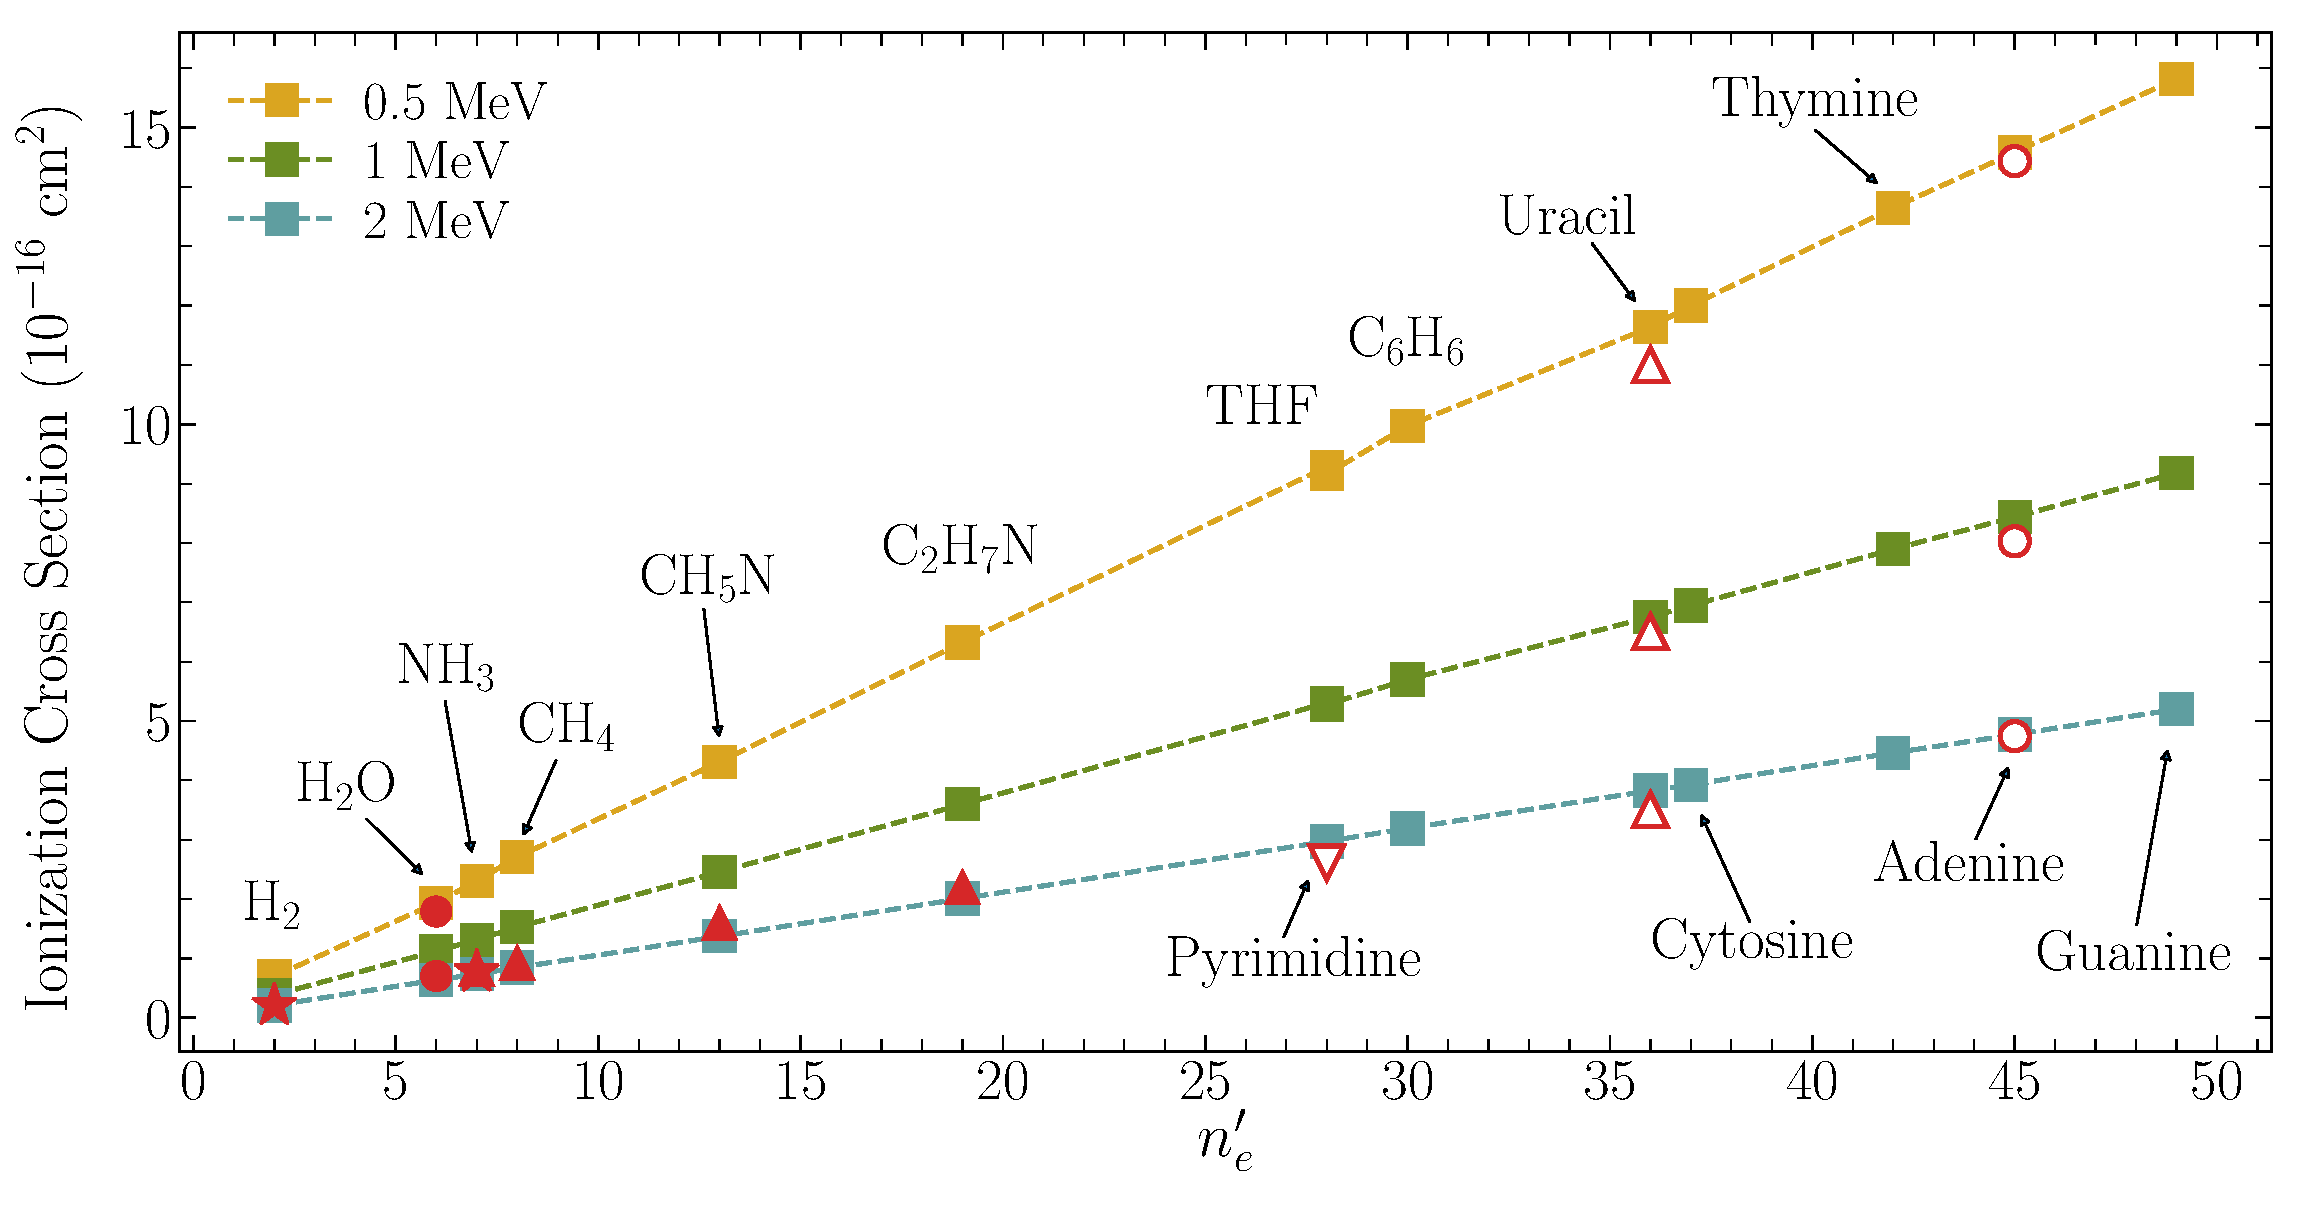
\includegraphics[width=0.9\textwidth]{ionmol/scale_ne.eps}
\caption[Sección eficaz de ionización por impacto de protón en términos de
$n_e$.]
{Sección eficaz de ionización por impacto de protón a 0.5, 1,
y 2 MeV en términos del númbero de electrones activos dado por la 
tabla~\ref{nn}. Experimentos: 
\mbox{\Large$\circ$}~adenina~\cite{iriki2011}, 
$\triangle$ uracilo~\cite{itoh2013}, 
$\bigtriangledown$ pirimidina~\cite{wolff2014}, 
$\blacktriangle$ C$_2$H$_7$N, CH$_5$N, metano y amoníaco~\cite{lynch1976},
\mbox{\scriptsize$\bigstar$} amoníaco y H$_2$~\cite{rudd1985}, y 
\mbox{\Large$\bullet$} agua~\cite{luna2007}.}
\label{fig:recta}
\end{figure}

Usando la ecuación~(\ref{eq:scalingCDW}), definimos nuevos números de 
electrones activos $n_e'$ para las moléculas consideradas. En la 
tabla~\ref{nn}, mostramos los nuevos valores $n_e'$ y los números de 
Toburen $n_e$, que resultan de aplicar la ecuación~(\ref{eq:nelec}). 
Nuestros resultados son diferentes a los propuestos por Toburen, los 
cuales son utilizados por otros autores~\cite{itoh2013}, principalmente 
debido a las diferencias en los números de electrones activos del 
oxígeno. Una forma alternativa de probar la escala propusta se puede
obtener dibujando las secciones eficaces de ionización de las moléculas 
en función de los valores dados para $n_e'$ según la tabla~\ref{nn}. 
Nuestros resultados se muestran en la figura~\ref{fig:recta} para 
energías de impacto de 0,5, 1 y 2 MeV. Como puede observarse, las 
secciones eficaces de ionización CDW calculadas para todas las moléculas 
muestran una dependencia lineal con el número de electrones $n_e'$ de 
la tabla~\ref{nn}. Obtenemos resultados similares, incluso para 
$E=10$~MeV. La comparación con los datos experimentales disponibles 
muestra una buena concordancia general, desde moléculas pequeñas, tales
como H$_2$, H$_2$O, and CH$_4$, hasta las más complejas, como la adenina. 
Para los datos de ionización por impacto de electrón, los datos 
experimentales se interpolaron entre vecinos cercanos. 
%It is worth mentioning that an equivalent plot using the Toburen numbers 
%$n_e$ does not exhibit the straight lines obtained with the present scaling. 

%While finishing the present work, we became aware of an accepted 
%manuscript by L\"udde~\textit{et al.}~\cite{ludde2019} on total 
%ionization of biological molecules by proton impact, using the
%independent--atom--model pixel counting method~\cite{ludde2016,ludde2018}.
%The authors also raised a scaling  with $\nu_{\alpha}=4$ for C, N, and O, 
%but $\nu_{\alpha}=6$ for P. The agreement with this independent method 
%for proton impact reinforces our multicharged--ion findings.

%%%%%%%%%%%%%%%%%%%%%%%%%%%%%%%%%%%%%%%%%%%%%%%%%%%%%%%%%%%%%%%%%%%%%%%%
\section{Estructura molecular de los blancos}
\label{sec:molcalculations}
%%%%%%%%%%%%%%%%%%%%%%%%%%%%%%%%%%%%%%%%%%%%%%%%%%%%%%%%%%%%%%%%%%%%%%%%

Finalmente, para probar el rango de validez del SSM, realizamos un 
cálculo molecular de primeros principios para cinco nucleobases 
empleando el código {\sc gamess}. La optimización de la geometría y los 
cálculos de energía de un centro se realizaron implementando el método
restringido de Hartree-Fock y el conjunto de bases 3-21G. 

\begin{figure*}[t]
\centering
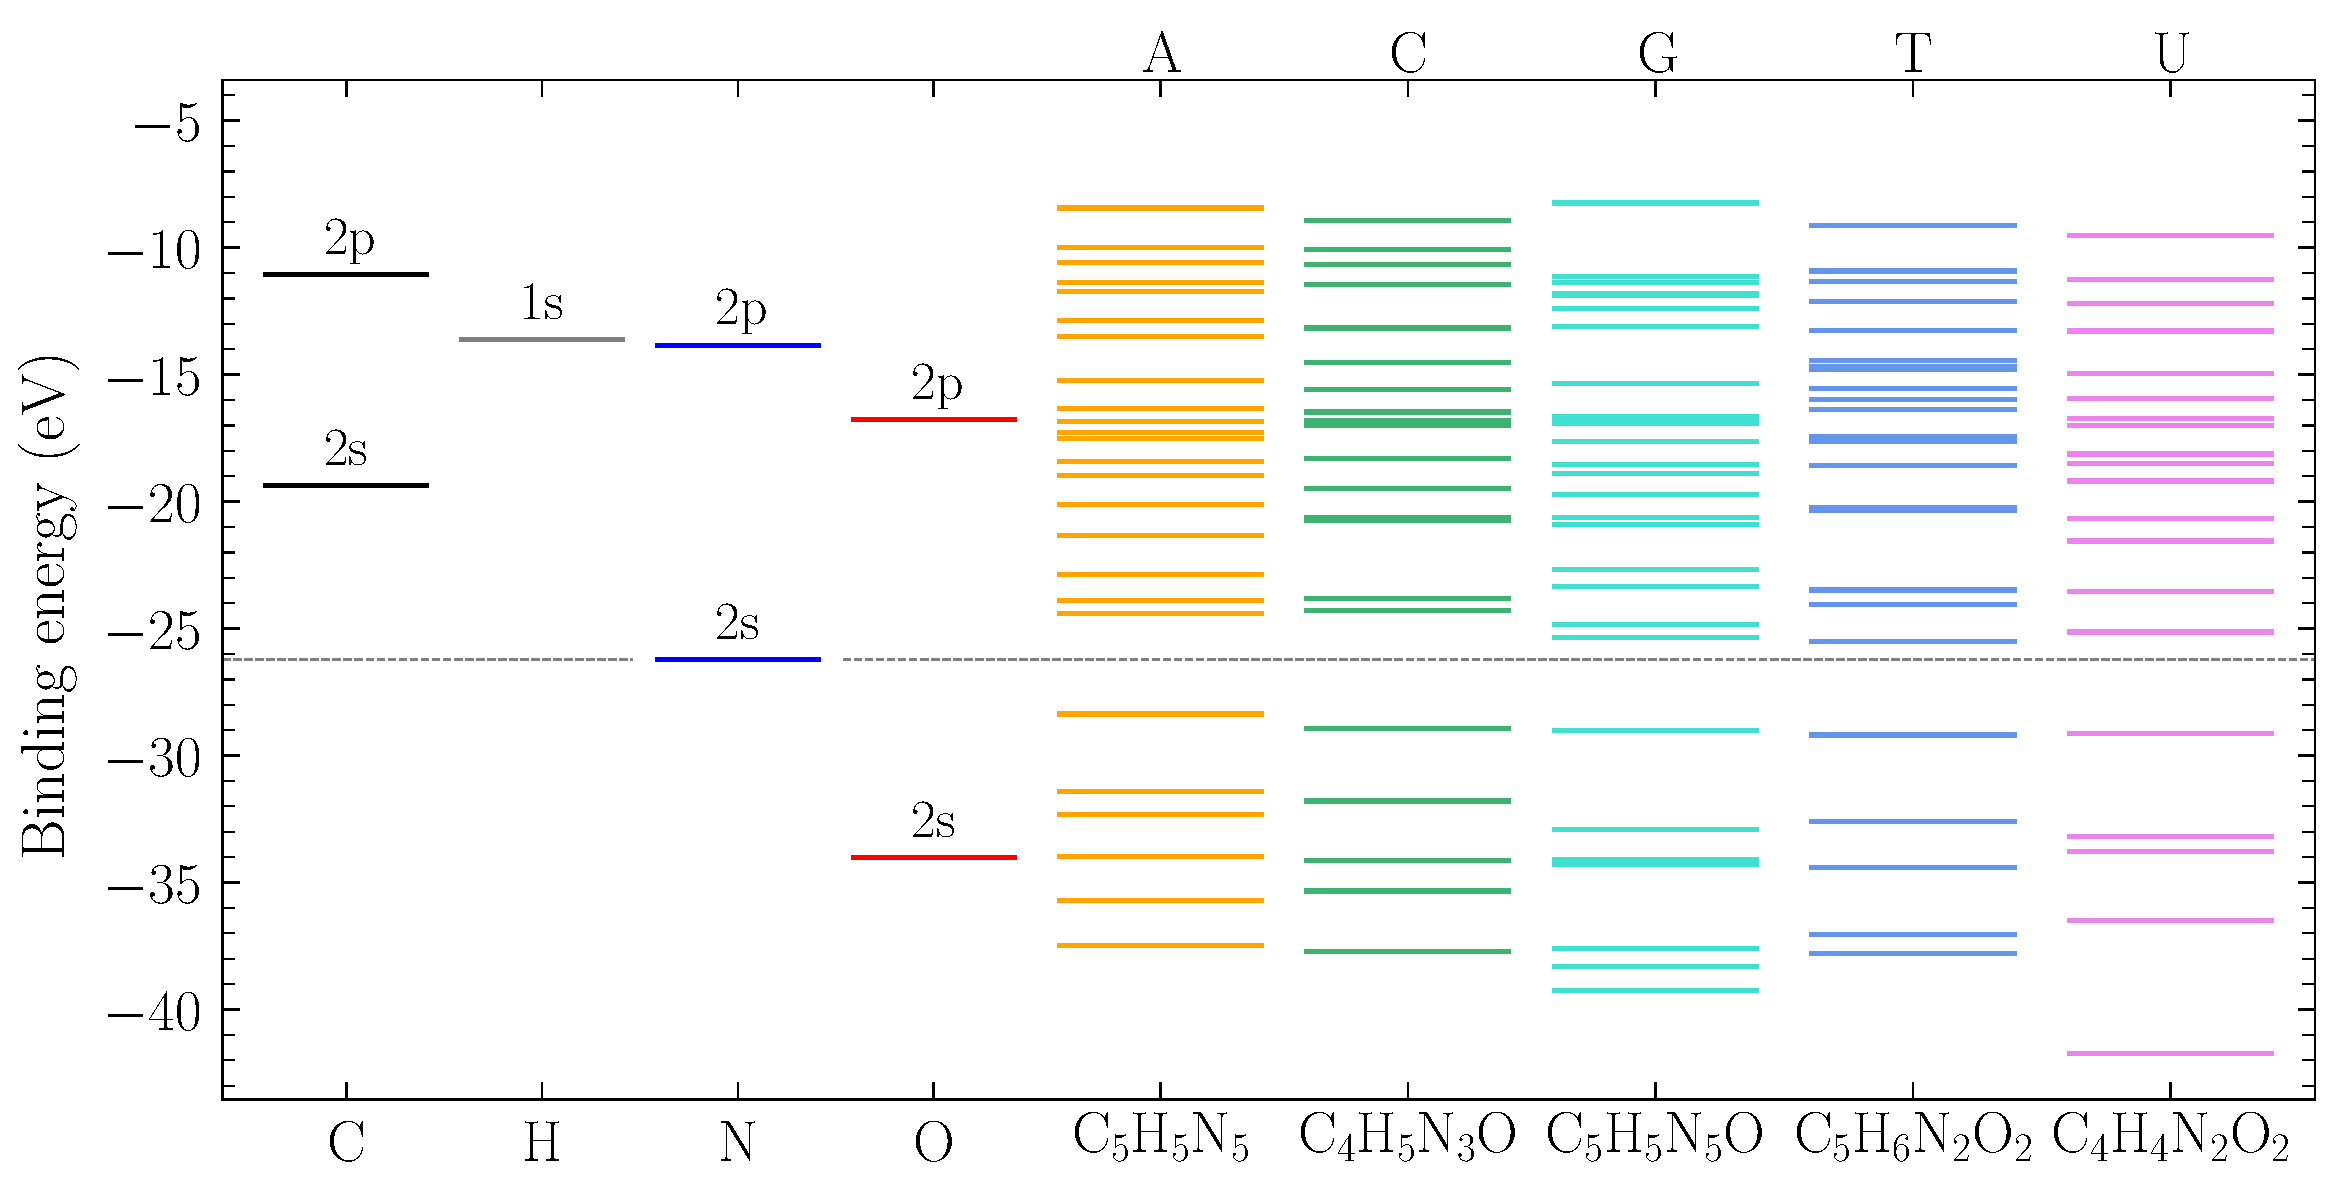
\includegraphics[width=\textwidth]{ionmol/levelsDNA.eps}
\caption[Energías de ligadura moleculares teóricas de ADN y ARN.]
{Energías de ligadura moleculares teóricas de adenina, citosina, guanina, 
timina, y uracilo, comparado con los valores correspondientes de los 
átomos que las constituyen.}
\label{fig:bindener}
\end{figure*}

En la figura~\ref{fig:bindener} se muestran las energías de ligadura 
molecular de los electrones de valencia para las nucleobases: adenina, 
citosina, guanina, timina y uracilo. Las energías de ligadura del orbital 
molecular más alto (HOMO) obtenidos concuerda con los valores
experimentales~\cite{Hush,Verkin,Dougherty} en un 2\% para todas las 
moléculas consideradas. En el lado izquierdo de la figura~\ref{fig:bindener}, 
mostramos las energías atómicas de Hartree-Fock de los elementos 
constituyentes, lo que da una idea de la distribución de los electrones
débilmente ligados en las moléculas. Se traza una línea discontinua 
alrededor de $-26$~eV para separar la banda molecular en dos. Podemos 
considerar los niveles de energía atómica por encima de esta línea como 
los correspondientes a los electrones débilmente ligados de la 
ecuación~(\ref{eq:scalingCDW}). Por ejemplo, los electrones $2s$ y $2p$ 
del carbono se ubican por encima de la línea discontinua, que corresponde 
a los 4 electrones dados por la escala CDW. En el caso de O, solo 4 
electrones de los orbitales 2p se encuentran por encima de la línea 
divisoria propuesta, que se corresponde con el número de electrones
débilmente ligados dado por el escaleo CDW. El caso del átomo de N no 
es tan directo; el número $\nu_{N=4}^{\text{CDW}}$ sugiere que uno de 
los dos electrones de la capa $2s$ contribuye al esquema molecular.

%%%%%%%%%%%%%%%%%%%%%%%%%%%%%%%%%%%%%%%%%%%%%%%%%%%%%%%%%%%%%%%%%%%%%%%%
\subsection{Un modelo estequiométrico modificado}
%%%%%%%%%%%%%%%%%%%%%%%%%%%%%%%%%%%%%%%%%%%%%%%%%%%%%%%%%%%%%%%%%%%%%%%%

El modelo estequiometrico simple considera a la molécula como un 
conjunto de átomos neutrales aislados, lo cual es definitivamente irreal.
Una primera mejora se puede sugerir asumiendo que los átomos no son
efectivamente neutrales y que tienen una distribución dispar de los 
electrones dentro de la molécula, lo cual puede expresarse mediante una
carga efectiva $q_{\alpha}$ por átomo. La carga de Mulliken proporciona
un valor posible para $q_{\alpha}$; sin embargo, existe una gran variedad
de posibles distribuciones de carga~\cite{lee2003}.

\begin{table*}[t]
\begin{center}
\begin{tabular}{|p{0.12\textwidth}|p{0.08\textwidth}|p{0.08\textwidth}|p{
0.08\textwidth}|p{0.08\textwidth}|p{0.24\textwidth}|}
\hline
Element & C & H & N & O & New stoichiometry \\
\hline
Adenine & +0.32 & +0.23 & --0.55 &       & 
C$_{4.92}$H$_{4.77}$N$_{5.14}$ \\ 
\hline
Cytosine & +0.28 & +0.21 & --0.56 & --0.53 & 
C$_{3.93}$H$_{4.79}$N$_{3.14}$O$_{1.13}$ \\ 
\hline
Guanine & +0.46 & +0.20 & --0.58 & --0.36 & 
C$_{4.89}$H$_{4.80}$N$_{5.15}$O$_{1.09}$ \\ 
\hline
Thymine & +0.20 & +0.19 & --0.54 & --0.52 & 
C$_{4.95}$H$_{5.81}$N$_{2.13}$O$_{2.13}$ \\ 
\hline
Uracil & +0.31 & +0.22 & --0.59 & --0.47 & 
C$_{3.92}$H$_{3.78}$N$_{2.15}$O$_{2.12}$ \\ 
\hline
\end{tabular}
\caption[Cargas efectivas medias de Mulliken por átomo]
{Cargas efectivas medias de Mulliken por átomo $q_{\alpha}$, y nueva formula
estequiométrica definida por la ecuación~(\ref{eq:newstoi}) para cinco
moléculas de ADN.}
\label{tab:newstoi}
\end{center}
\end{table*}

Para tomar en cuenta este efecto, consideramos que el número total de 
electrones $Q_{\alpha }$ en el elemento $\alpha$ se distribuye de forma
dispar sobre todos los átomos $\alpha$. Por lo tanto, cada elemento  
$\alpha$ tendrá una carga adicional, $q_{\alpha}=Q_{\alpha}/n_{\alpha}$, 
que puede ser positiva o negativa. Esta valor dependerá de la 
electronegatividad relativa respecto a los otros átomos~\cite{rappe1991}. 
Siguiendo esta idea, podemos estimar el nuevo número de átomos por 
molécula $n_{\alpha }^{\prime }$, el cual está dado por
\begin{equation}
n_{\alpha }^{\prime }=n_{\alpha }-
\frac{q_{\alpha }}{\nu_{\alpha }^{\text{CDW}}}
\label{eq:newstoi}
\end{equation}
En el caso de átomos neutrales, $q_{\alpha}=0$ y 
$n_{\alpha}^{\prime}=n_{\alpha}$, como debería ser. En la 
tabla~\ref{tab:newstoi}, mostramos un valor promedio de carga efectiva por
átomo $q_{\alpha}$ de C, H, N, y O, para cinco moléculas del ADN,
las cuales se obtuvieron a partir de los cálculos moleculares descritos 
en la sección anterior.

Implementando la ecuación~(\ref{eq:newstoi}), es posible determinar
una nueva fórmula estequiométrica, la cual se da en la última columna de
la tabla~\ref{tab:newstoi}). Ahora, en vez de tener un número entero 
de átomos $n_{\alpha}$, tenemos un número fraccional dado por 
$n_{\alpha}^{\prime}$. Se pueden calcular nuevas secciones eficaces 
moleculares, $\sigma^{\prime}_{M}=\sum_{\alpha}n_{\alpha}'\sigma_{\alpha}$
considerando tales valores. Se calcularon errores relativos de las 
secciones eficaces de ionización para las bases de ADN de la 
tabla~\ref{tab:newstoi}. Las diferencias obtenidas fueron menores de
3\%, lo cual indica que el modelo estequiométrico simple 
es un modelo robusto con el que se pueden modelar este tipo de 
moléculas complejas dentro del margen de error esperado.

%%%%%%%%%%%%%%%%%%%%%%%%%%%%%%%%%%%%%%%%%%%%%%%%%%%%%%%%%%%%%%%%%%%%%%%%
\section{Conclusiones}
%%%%%%%%%%%%%%%%%%%%%%%%%%%%%%%%%%%%%%%%%%%%%%%%%%%%%%%%%%%%%%%%%%%%%%%%

En este capítulo, hemos estudiado la ionización de blancos moleculares 
de interés biológico debido al impacto de iones de carga múltple. Se han
calculado secciones eficaces de ionización de diesciseis blancos 
moleculares biological conteniendo H, C, N y O por el impacto de
antiprotones, H$^{+}$, He$^{2+}$, Be$^{4+}$, C$^{6+}$, y O$^{8+}$. 
Hemos combinado la implementación del método de onda distorcionada
CDW para blancos atómicos descritos con potenciales efectivos DIM y la 
estructura molecular fue modelada con un simple modelo estequiométrico.
También se estudiaron y calcularon los valores medios de energía y 
ángulo de emisión de los electrones ionizados de los blancos atómicos, 
que son de importancia en el daño secundario de las colisiones con iones.
Nuestros resultados muestran una clara dependencia de estos valores con 
la carga del ion $Z$. Para un blanco dado, a medida que $Z$ aumenta,
$\overline{E}_{\alpha}$ también aumentan. Por otro lado, 
$\overline{\theta}_{\alpha}$ decrece, lo que muestra una clara tendencia 
a la dirección del ion. A energía de impacto mayores a 2 MeV/amu, estos
valores convergen a la primera aproximación de Born, la cual establece 
la simple ley de escala $Z^{2}$. 

También se presentaron secciones eficaces de ionización total
para adenina, citosina, timina, guanina, uracilo, esqueleto de DNA, 
pirimidina, y THF, siendo comparadas a su vez con los pocos datos
experimentales disponibles. Explarmos la ampliamente usada regla de 
escala de Toburen, que escala la sección eficaz de ionización molecular 
con un determinado número de electrones débilmente ligados.
Encontramos que las secciones eficaces de ionización escalan
mejor cuando se normalizan con diferentes números de electrones activos
en la colisión, los cuales son obtenidos a partir de los resultados CDW
para los atómos H, C, N y O. Esta nueva regla de escala fue 
probada con buenos resultados para los seis proyectiles y diecisiete 
moléculas estudiadas aquí. La comparación con los datos experimentales 
refuerza nuestros hallazgos. Además, probamos la escala mediante la 
inclusión de datos experimentales de ionización de H$_2$, agua, metano 
y amoníaco por impacto de protones, los cuales muestran una buena 
concordancia a energías intermedias a altas.

Finalmente, realizamos cálculos moleculares completos para las 
nucleobases del ADN. Al inspeccionar las energías de ligadura 
moleculares obtenidas mediante cálculos mecanicocuánticos de primeros 
principios, pudimos comprender el número de electrones propuestos en 
nuestro nuevo escaleo basado en los cálculos CDW. Intentamos mejorar el 
modelo estequiométrico utilizando la carga de Mulliken para obtener 
proporciones fraccionarias en lugar de enteras. No encontramos una 
corrección sustancial, lo que indica que el SSM funciona bastante bien. 
En conclusión, los presentes resultados refuerzan la exactitud del modelo
estequiométrico simple para tratar con moléculas complejas en el rango 
de energía intermedia a alta. 



